\documentclass{article}

\usepackage[a4paper, top=2cm, bottom=3cm]{geometry}

\usepackage[ngerman]{babel}
\usepackage{csquotes}

\usepackage{booktabs}
\usepackage{mathtools}
\usepackage{amssymb}
\usepackage{enumitem}
\usepackage{amsmath}

\usepackage{hyperref}

\usepackage{graphicx}
\usepackage{wrapfig}

\usepackage{pgfplots}
\pgfplotsset{compat=1.18}

\usepackage{siunitx}
\sisetup{locale = DE}

\usepackage{biblatex}
\DefineBibliographyStrings{ngerman}{
  urlseen = {Abruf vom}
}
\addbibresource{quellen.bib}

\newcommand{\proofeq}{\overset{!}{=}}
\newcommand{\proofeqv}{\overset{!}{\Leftrightarrow}}
\newcommand{\equivalent}{\overset{\scriptscriptstyle\wedge}{=}}
\DeclarePairedDelimiter\ceil{\lceil}{\rceil}
\DeclarePairedDelimiter\floor{\lfloor}{\rfloor}

\date{20.03.2022}
\title{Physikalisches Grundpraktikum Teil I \\ (Mechanik und Thermodynamik) \\ Versuch 2 Drehbewegung}
\author{Finn Bietz (8104485), Finn Wagner (8102237)}

\begin{document}

	\maketitle

	\section{Versuchsziel und Versuchsmethode}
	In diesem Experiment soll das Trägheitsmoment eines Kreisels bestimmt werden.
	Dazu werden drei unterschiedliche Versuche durchgeführt. Beim Ersten messen wir indirekt die Winkelbeschleunigung, beim Zweiten die Schwingungsdauer der Kreisscheibe
	und beim Dritten die Dauer der Präzessionsbewegung, sowie die währenddessen vollführten Eigenrotationen.
	Aus diesen Messungen errechnen wir dreimal das selbe Trägheitsmoment.

	\section{Allgemeiner Aufbau}
	Der Kreisel ist eine Scheibe die in ihrem Mittelpunkt auf eine Stab aufgesteckt ist. Die Scheibe kann um ihren Mittelpunkt frei rotieren.
	Der Stab wird im Schwerpunkt des Systems Scheibe-Stab mit einem Drehgelenk gestützt und auf der gegenüberliegenden Seite von einem Gegengewicht in Waage gehalten.
	Das Drehgelenk kann in alle Richtungen drehen. Zum fixieren des Gelenks steht in den ersten beiden Versuchen ein Stativ zur Verfügung.
	\begin{figure}[!ht]\label{fig:aufbau}
		\centering
		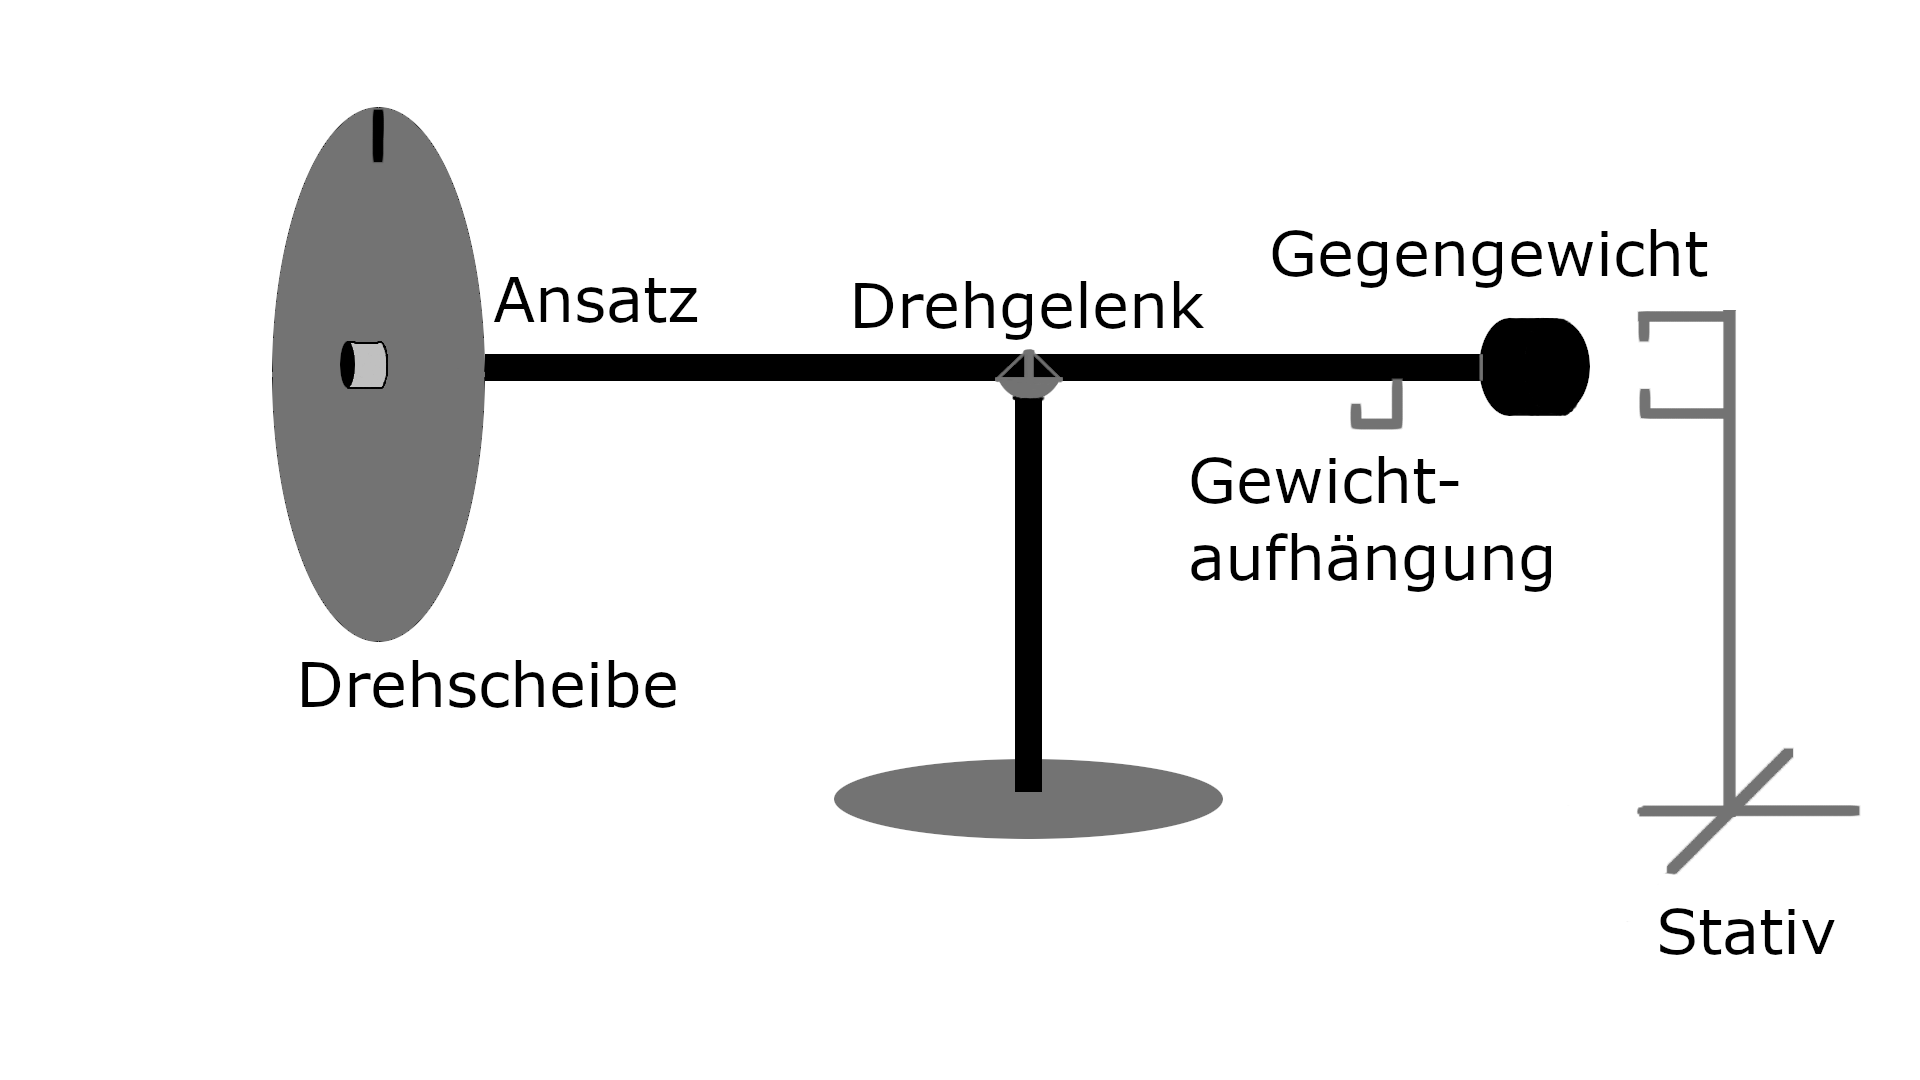
\includegraphics[width=\textwidth]{aufbau.png}
		\caption{Allgemeiner Versuchsaufbau}
	\end{figure}

	\section{Allgemeine Theorie}\label{Allgemeine_Theorie}
	Das Trägheitsmoment ist der Zusammenhang zwischen der kinetischen Rotationsenergie eines Körpers und seiner Winkelgeschwindigkeit, nach der Formel \(K = \frac{1}{2}I \omega^2\).
	Damit stellt es den gleichen Zusammenhang her wie die Masse bei translatorischen Bewegungen.
	Die Formeln \({K = \frac{1}{2} m v^2}\), sowie \({K = \frac{1}{2} I \omega^2} \) ähneln sich dabei stark.
	Auch ist es ein Maß für den Widerstand den ein Körper der Änderung seiner Rotationsbewegung entgegensetzt. \\
	Das Trägheitsmoment kann man für diskrete oder kontinuierliche Masseverteilungen bestimmen.
	Zunächst leiten wir es für diskrete Verteilungen her. Wir machen folgende Überlegungen.
	Für nur rotierende Körper ist die Summe aller Bewegungsenergien gleich aller Rotationsenergien.
	Zu einem diskreten Zeitpunkt lassen sich die Rotationen als geradlinige Bewegungen betrachten. Es gilt also:
	\begin{equation}
		K = \frac{1}{2} m_1 v_1^2 + \frac{1}{2} m_2 v_2^2 + \cdots = \sum \frac{1}{2} m_i v_i^2
	\end{equation}
	Wir ersetzen hier nun die Geschwindigkeit durch die Winkelgeschwindigkeit~\(\omega\) und den Radius~\(r\)
	(Kürzester Abstand zur Drehachse) mit \(v = \omega r\)
	\begin{equation}
		K = \sum \frac{1}{2} m_i {\left( \omega r_i \right)}^2 = \frac{1}{2} \left( \sum m_i r_i^2 \right) \omega^2
	\end{equation}
	Womit wir auf die Definition des Trägheitsmoments
	\begin{equation}\label{eq:trägheitsmoment_diskret}
		I = \sum m_i r_i^2
	\end{equation} kommen. Siehe~Quelle~\cite{HallidayPhysik} \\
	Um ein solches Trägheitsmoment anzugeben braucht man aber zwingend noch eine dazugehörige Drehachse.
	Die Winkelgeschwindigkeiten und Radien in der Herleitung werden alle bezogen auf die selben Achse angegeben.
	Bei krummen oder nicht symmetrischen Körpern kann man sich leicht visualisieren, dass ein verschieben der Achse einen großen Einfluss auf das Trägheitsmoment haben kann.
	Einen Stift entlang seiner langen Achse zu drehen fällt leicht, da die Masse des Stiftes nicht so weit von der Drehachse entfernt ist.
	Dreht man ihn um seine Spitze ist die Masse viel weiter von der Drehachse entfernt und das Trägheitsmoment damit merklich größer.
	Natürlich kann man das Trägheitsmoment auch für volle/dichte Körper berechnen. Man braucht hierfür die Massen-/ Dichteverteilung im Volumen. Die allgemeine Definition ist also:
	\begin{equation}
		I = \int_V \ \vec{r}_{\bot}^{\,2} \  \rho(\vec{r}) \ dV
	\end{equation}
	Man integriert also über das gesamte Volumen des betrachteten Körpers mit seiner Dichteverteilung und den Abstandsquadraten der Punkte zur betrachteten Drehachse. Diese Form ist der Grenzfall für unendlich viele Massestücke aus Definition~(\ref{eq:trägheitsmoment_diskret}).
	
	Hat man bereits ein Trägheitsmoment mit Drehachse durch den Massenmittelpunkt bestimmt, so lassen sich mit dem Steiner'schen Satz alle Trägheitsmomente von dazu parallel verschobenen Drehachsen berechnen.
	Man addiert dafür zu dem bereits bekannten Drehmoment \(I\) den Term \(m \cdot r^2\) hinzu (Siehe~\cite{Steiner}). Hieraus erkennt man sofort, dass das Drehmoment einer Achse die nicht
	durch den Schwerpunkt geht, immer echt größer ist als der Achse von \(I\),
	da man durch anwenden des Steiner'schen Satzes immer etwas positives hinzuaddiert.
	
	Das Trägheitsmoment eines aus mehreren Teilkörpern zusammengesetzten Objekts lässt sich durch addieren der einzelnen Teilträgheitsmomente zur gleichen Achse berechnen.
	Dafür kann man das Trägheitsmoment eines Teilkörpers gesondert berechnen und dann, mit Hilfe des Steiner'schen Satzes, auf die richtige Achse verschieben.
	Dieser Eigenschaft ist sehr praktisch, da viele Trägheitsmomente bereits berechnet sind und sich in Refernztabellen, wie z.B. in Quelle~\cite{HallidayPhysik} finden lassen.
	
	Das Trägheitsmoment wird nicht nur für die Energieberechnung verwendet, sondern auch hier wieder ähnlich zur Masse, für den Drehimpuls \(L = I \omega \) und das Drehmoment \(M = I \alpha \).
	Trägheitsmomente eines Körpers lassen sich auch über einen Trägheitstensor ausdrücken, mit dessen Hilfe sich das Trägheitsmoment zu einer beliebigen Achse einfach berechnen lässt. \\
	Für die Intuition sei hier noch angefügt, dass je kleiner das Trägheitsmoment eines Körpers um eine Achse ist, desto leichter lässt er sich um sie drehen~\cite{HallidayPhysik}.

	\section{Trägheitsmoment über die Winkelbeschleunigung}

	\subsection{Durchführung}
	\subsubsection{Materialien}
	\begin{itemize}
		\item Kreisel (siehe allgemeiner Aufbau)
		\item kleines Gewicht (\(\approx \SI{100}{\gram}\))
		\item Schnur mit einer Länge von \(\approx \SI{1,5}{\metre} \)
		\item Waage
		\item Stoppuhr (Handy)
		\item Schieblehre
	\end{itemize}
	\subsubsection{Versuchsdurchführung}

	\begin{enumerate}
		\item Masse \(m\) des Gewichts zusammen mit Faden messen.
		\item Messen des Radius der Schnuraufwicklung (Zylindrischer Ansatz an der Vorderseite der Scheibe) mit der Schieblehre.
		\item Aufwickeln des Fadens und anhängen des Gewichts an die Kreisscheibe.
		\item Messen Sie nun die für eine komplette Umdrehung benötigten Zeiten \(t_R\) mit der \enquote{Runden}-Funktion der Smartphone Stoppuhr.
	\end{enumerate}
	
	Für diesen Versuch wollen wir auf die Scheibe ein konstantes Drehmoment wirken lassen.
	Dies wird durch das Anhängen eines kleinen Gewichts der Masse \(m\) mit einer Schnur an einen hervorstehenden Zylinder erreicht.
	Die Schnur, an welcher das Gewicht hängt, wird auf diesen Zylinder aufgewickelt (Abb.~\ref{fig:Angehängte Masse}). \\
	Nun wird das Gewicht losgelassen, worauf hin das durch das Gewicht erzeugte Drehmoment die Scheibe in Rotation versetzt.
	Die Rotation wird durch das konstant wirkende Drehmoment konstant weiter beschleunigt, sodass die Scheibe sich immer schneller dreht, also eine immer kürzer werdende Zeit für jede Umdrehung braucht. \\
	Wir messen nun die Zeit \(t_R\), welche die Scheibe für eine Umdrehung benötigt.
	Eine Umdrehung der Scheibe erkennen wir daran, dass die Markierung wieder in ihre Ausgangslage zurück rotiert ist.
	Die Zeiten werden per Hand mit einer Handystoppuhr gemessen. Für jede Umdrehung messen wir mit der \enquote{Rundenzeiten} Funktion der Stoppuhr-App die Umdrehungszeit.
	Es werden so lange Zeiten gemessen, bis der Faden komplett abgewickelt ist. Es ist darauf zu achten, dass das Gewicht nicht bereits wieder hoch gezogen wird und die Scheibe abbremst. \\
	Die Masse \(m\) wird mit einer Waage gemessen, wobei der Faden, mit dem sie angehängt wird mitgewogen wird. \\
	Der Radius des Zylinders, an den die Masse angehängt wird, wird mit einer Schieblehre bestimmt.

	\begin{figure}[!ht]
		\centering
		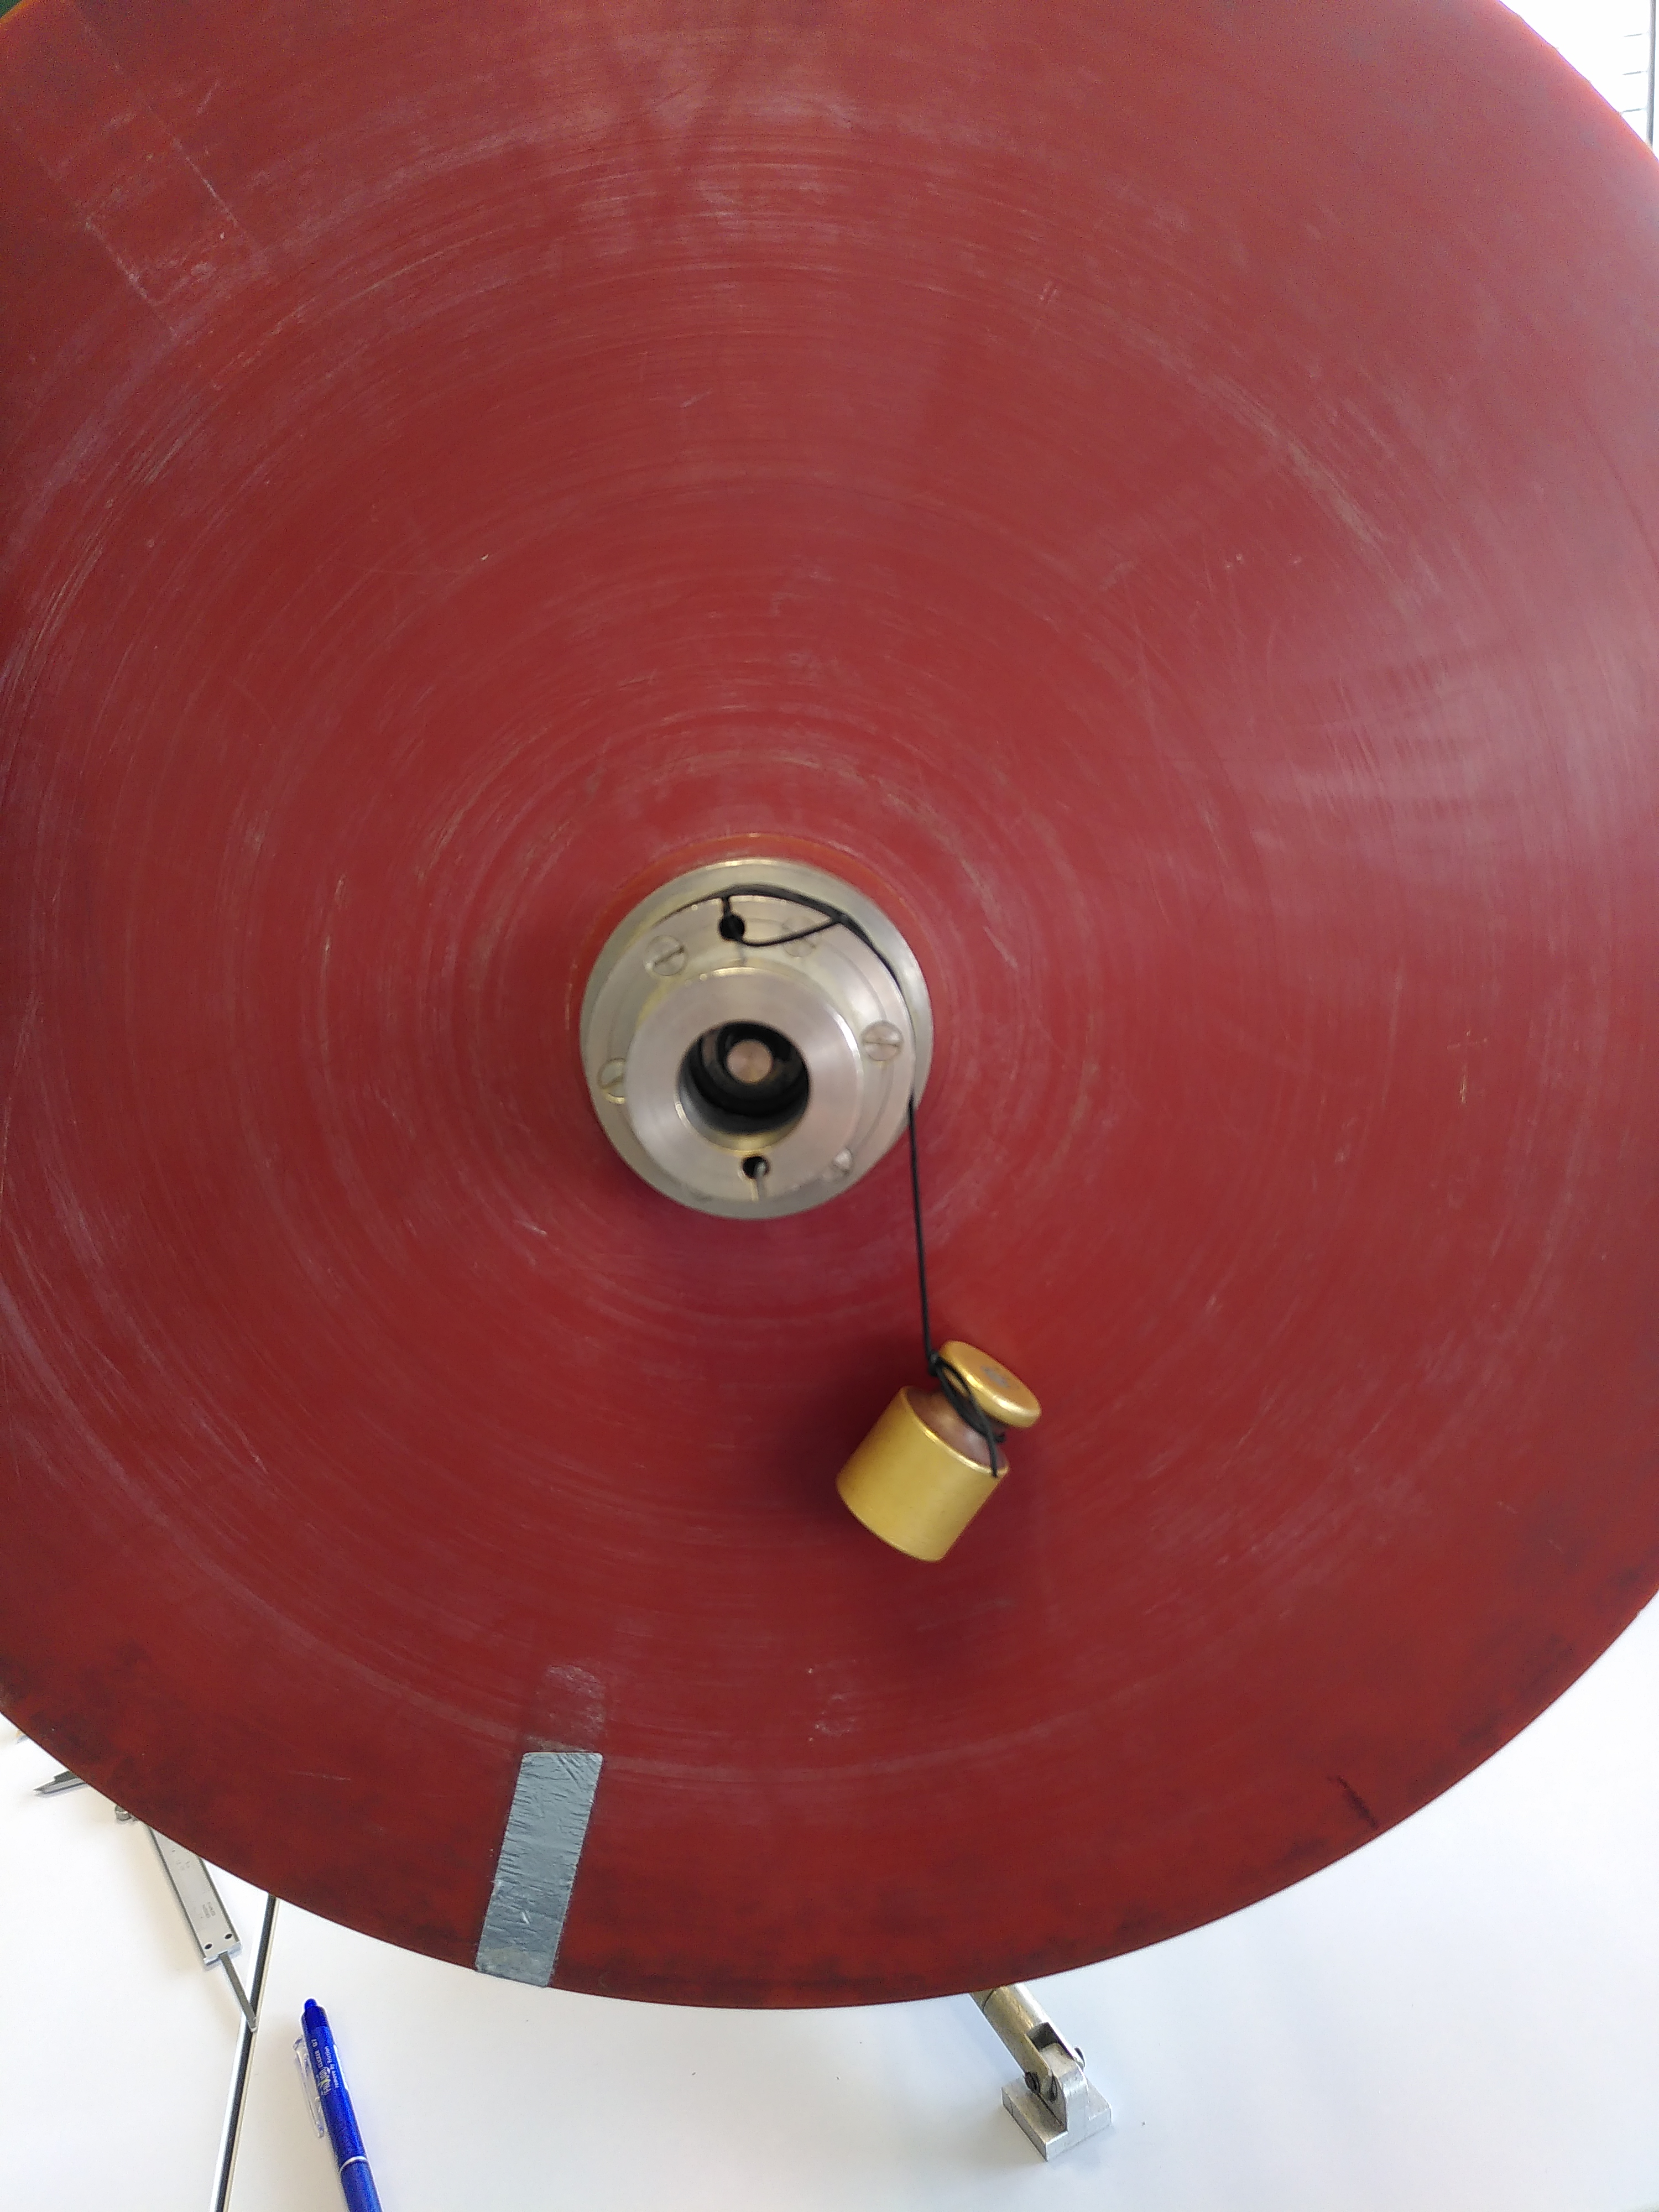
\includegraphics[width=0.5\textwidth]{Winkelbeschleunigung.jpg}
		\caption{\label{fig:Angehängte Masse}Die Masse angehängt an den Zylinder}
	\end{figure}

	\subsection{Messergebnisse}
	Mit Hilfe der Waage wurde die Masse des kleinen Gewichts \(m\) auf \(\SI{99}{\gram}\) bestimmt. \\
	Die benutzte Waage hat eine Genauigkeit von einem Gramm.
	Die Schnuraufwicklung hat den Durchmesser (Durchmesser des Zylinders) \(d = \SI{4.93}{cm}\). (Diesen Messwert haben wir bei den Messergebnissen im Anhang fälschlicherweise als Radius bezeichnet).
	Die dazu verwendete Schieblehre hat eine Genauigkeit von \(\SI{0.05}{mm}\). \\
	Für die Messungen wurde eine Handystoppuhr verwendet mit einer Genauigkeit von einer Millisekunde. {\Huge Centisekunde} %TODO:
	Der Winkel wurde mit dem Auge geschätzt. \\

	\subsubsection{Winkel und Zeiten}
	\begin{table}[!ht]
		\centering
		\begin{tabular}{ | c | c | }
			\hline
			Winkel \( \varphi \) & Rundenzeit \(t_R [\unit{\second}]\) \\
			\hline
			\( 2\pi \)           & 4,89 \\
			\( 4\pi \)           & 2,14 \\
			\( 6\pi \)           & 1,67 \\
			\( 8\pi \)           & 1,33 \\
			\( 10\pi \)          & 1,21 \\
			\hline
		\end{tabular}
		\caption{Winkel und Rundenzeiten}
	\end{table}

	Damit ergibt sich für die Winkel und die insgesamt verstrichene Zeit:
	\begin{table}[!ht]
		\centering
		\begin{tabular}{ | c | c | }
			\hline
			\( \varphi \) & \(t [\unit{\second}]\) \\
			\hline
			\( 2\pi \)    & 4,89 \\
			\( 4\pi \)    & 7,03 \\
			\( 6\pi \)    & 8,70 \\
			\( 8\pi \)    & 10,03 \\
			\( 10\pi \)   & 11,24 \\
			\hline
		\end{tabular}
		\caption{\label{tab:Winkel_Gesamtzeit}Winkel und Gesamtzeit}
	\end{table} \\
	Messwerte aus (\ref{fig:Messwerte1}).

	\subsection{Auswertung}
	\subsubsection{Formeln}
	Durch anhängen des Gewichts mit der Masse \(m\) an den aufgewickelten Faden erzeugt man ein Drehmoment \(M = m g r\), wodurch die Scheibe eine konstante Winkelbeschleunigung erfährt.
	\begin{equation} \label{eq:Drehmoment}
		M = I \alpha = I \frac{d\omega}{dt}
	\end{equation}
	Zwischen dem Winkel und der Winkelbeschleunigung \( \alpha \) besteht die Beziehung:
	\begin{equation} \label{eq:Beschleunigter_Winkel}
		\varphi = \frac{1}{2} \alpha t^2
	\end{equation}
	Sie gilt, wenn die Scheibe mit Winkelgeschwindigkeit und Winkel 0 beginnt \(\omega = \varphi = 0\).
	Hier gegeben, da die Scheibe zu Beginn des Experiments in Ruhe ist.
	Setzen wir die Formel~\ref{eq:Beschleunigter_Winkel} nach \( \alpha \) umgeformt in Formel~\ref{eq:Drehmoment} ein, so folgt:
	\begin{equation}
		I = \frac{M}{\alpha} = \frac{ Mt^2 }{2 \varphi}
	\end{equation}
	Das Drehmoment wird durch das am Faden hängende Gewicht erzeugt. Es erzeugt wegen der Art seiner Aufhängung immer das Drehmoment \( M = m g r \). Setzen wir ein folgt:
	\begin{equation}
		I = \frac{ m g r \cdot t^2 }{ 2 \varphi }
	\end{equation}
	Hier können wir noch einen Teil durch die Steigung \(S = \frac{ \varphi }{ t^2 } \) und den Radius \(r = \frac{d}{2}\) ersetzen:
	\begin{equation}\label{eq:Trägheitsmoment_komplett}
		I = \frac{mgd}{4S}
	\end{equation}

	\subsubsection{Graphische Auswertung}
	In Gleichung (\ref{eq:Beschleunigter_Winkel}) erkennen wir den linearen Zusammenhang zwischen \( \varphi \) und \( t^2 \).
	Tragen wir also die gemessenen Werte für \( \varphi \) und \( t^2 \) in ein Koordinatensystem ein, sehen wir eine Gerade, weil die beiden Größen einfach proportional zueinander sind.
	Wir rechnen unsere Messwerte aus Tabelle~\ref{tab:Winkel_Gesamtzeit} um, indem wir die Zeiten quadrieren.
	\begin{center}
		\begin{tabular}{ | c | c | }
			\hline
			\( \varphi \) & \(t^2 [\unit{\second^2}] \) \\
			\hline
			\( 2\pi \)    & 23,91 \\
			\( 4\pi \)    & 49,42 \\
			\( 6\pi \)    & 75,69 \\
			\( 8\pi \)    & 100,60 \\
			\( 10\pi \)   & 126,33 \\
			\hline
		\end{tabular}
	\end{center}
	Diese Werte werden in ein Diagramm eingetragen (Abbildung \ref{fig:Diagramm}), und die Steigung \( S = \frac{\varphi}{t^2} \) der Geraden, welche per Hand an die Datenpunkte gefittet wurde, wird bestimmt. Dazu werden zwei Punkte ausgewählt:
	\begin{equation}
		\begin{gathered}\label{eq:punkte}
			P_1: t^2_1 = 20s^2 ; \varphi_1 = 1,7 \pi \\
			P_2: t^2_2 = 130s^2 ; \varphi_2 = 10,3 \pi
		\end{gathered} % TODO: Wie wurde die Gerade gezeichnet
	\end{equation}
	Damit ergibt sich für \( S \):
	\begin{equation}
		S = \frac{ \varphi_2 - \varphi_1 }{ t^2_2 - t^2_2 } = \frac{ 10,3 \pi - 1,7 \pi }{ \SI{130}{\second^2} - \SI{20}{\second^2} } = \SI{0,2456}{\frac{1}{\second^2}}
	\end{equation}
	\begin{figure}
		\centering
		\includegraphics[width=1\textwidth]{Phi(t^2).png}
		\caption{\label{fig:Diagramm}$t^2$-$\varphi$-Diagramm}
	\end{figure}

	\subsubsection{Trägheitsmomentberechnung}
	Zur Berechnung des Ergebnisses setzen wir die Steigung \(S = \SI{0,2456}{\frac{1}{\second^2}} \), das Gewicht der beschleunigenden Masse \(m = \SI{99}{\gram} = \SI{0.099}{\kilogram}\), die Erdbeschleunigung
	\(g = \SI{9,81}{\frac{m}{s^2}} \), sowie den Radius der Aufhängung \(r = \SI{4.93}{cm} = \SI{0.0493}{\metre}\) in Gleichung (\ref{eq:Trägheitsmoment_komplett}) ein:
	\begin{equation}
		I = \frac{ \SI{0,099}{\kilogram} \cdot \SI{9,81}{\frac{m}{s^2}} \cdot \SI{0,0493}{m} }{ 4 \cdot \SI{0,2456}{\frac{1}{s^2}} } = \SI{0,0487}{\kilogram \cdot \metre^2}
	\end{equation}

	\subsubsection{Fehlerrechnung}
	% TODO: Abweichung bei Null
	Nun muss noch der maximale Fehler von \( I \) bestimmt werden, dieser ist gegeben als (Aufgabenstellung~\cite{AnleitungPraktikum}):
	\begin{equation}
		\Delta I =
		\left| \frac{\partial I}{\partial m} \right| \Delta m +
		\left| \frac{\partial I}{\partial d} \right| \Delta d +
		\left| \frac{\partial I}{\partial S} \right| \Delta S
	\end{equation}
	Wir berechnen zunächst die partiellen Ableitungen von Gleichung (\ref{eq:Trägheitsmoment_komplett}):
	\begin{equation}
		\begin{aligned}
			\frac{\partial I}{\partial m} & = \frac{\partial}{\partial m} \frac{m g r}{4S} = \frac{g r}{4S}     \\
			\frac{\partial I}{\partial d} & = \frac{\partial}{\partial d} \frac{m g d}{4S} = \frac{m g}{4S}     \\
			\frac{\partial I}{\partial S} & = \frac{\partial}{\partial S} \frac{m g r}{4S} = -\frac{m g r}{4S^2} \\
		\end{aligned}
	\end{equation}
	Wir setzen die partiellen Ableitungen in die Formel ein:
	\begin{equation}
		\Delta I =
		\left| \frac{g d}{4S} \right| \Delta m +
		\left| \frac{m g}{4S} \right| \Delta d +
		\left| -\frac{m g d}{4S^2} \right| \Delta S
	\end{equation}

	\paragraph{Graphischer Fehler} 
	Zunächst bestimmen wir \( \Delta S \), den Fehler der graphischen Darstellungen:
	\begin{equation}
		\frac{\Delta S}{S} = \frac{ 2 \Delta t^2 }{t^2_2 - t^2_1}
	\end{equation}
	Aus Kapitel 0.2.2.4 von Quelle~\cite{AnleitungPraktikum}.
	Wobei \( \Delta t^2 \) die größte Abweichung eines Messwertes von der Geraden bezeichnet.
	Bei unseren Messwerten ist das, das Wertepaar \( t = \SI{75,69}{\second} \); \( \varphi = 6\pi \).
	Hier weicht \( t^2 \) um \( \SI{1}{\second^2} \) von der gezeichneten Geraden ab.
	Mit \( t^2_1 \), \( t^2_2 \) von \( P_1 \) und \( P_2 \) (\ref{eq:punkte}) beträgt der Fehler von \( S \):
	\begin{equation}
		\Delta S = \frac{2\cdot 1s^2}{130s^2 - 20s^2}0,2456\frac{1}{s^2} = 0,0045\frac{1}{s^2}
	\end{equation}

	\paragraph{Maximaler Fehler}
	Der maximale Fehler der Waage, mit welcher \(m\) bestimmt wurde beträgt \(\Delta m = \SI{1}{\gram} = \SI{0.001}{\kilogram}\),
	und der Fehler der Schieblehre liegt bei \( \Delta d = \SI{0,05}{mm} = \SI{5e-5}{\metre} \).
	Somit ergibt sich für \( \Delta I \), mit einsetzen aller Messfehler und Variablen:
	\begin{equation}
		\begin{aligned}
			\Delta I = & \left| \frac{ \SI{9,81}{\frac{\metre}{\second^2}} \cdot \SI{0,0493}{\metre} }{ 4 \cdot \SI{0,2456}{\frac{1}{\second^2}} } \right| \cdot \SI{0,001}{\kilogram}                                           \\
			+          & \left| \frac{ \SI{0,099}{\kilogram} \cdot \SI{9,81}{\frac{\metre}{\second^2}} }{ 4 \cdot \SI{0,2456}{\frac{1}{\second^2}} } \right| \cdot \SI{5e-5}{\metre}                                             \\
			+          & \left| - \frac{ \SI{0,099}{\kilogram} \cdot  \SI{9,81}{\frac{\metre}{\second^2}} \cdot \SI{0,0493}{\metre} }{ 4 \cdot {(\SI{0,2456}{\frac{1}{\second^2}})}^2 } \right| \cdot \SI{0,0045}{\frac{1}{s^2}} \\
			=          & \SI{1,44e-3}{ \kilogram \cdot \metre^2 }
		\end{aligned}
	\end{equation}

	\subsubsection{Endergebnis}
	Das Trägheitsmoment beträgt bei der Bestimmung über die Winkelbeschleunigung also:
	\begin{equation}
		I = \SI{4,87e-2}{ \kilogram \cdot \metre^2 } \pm \SI{0,144e-2}{ \kilogram \cdot \metre^2 }
	\end{equation}

	\section{Trägheitsmoment über die Schwingungsdauer einer Pendelbewegung}

	\subsection{Durchführung}
	\subsubsection{Materialien}
	\begin{itemize}
		\item Kreisel (siehe allgemeiner Aufbau)
		\item Gewicht, welches sich an die Drehscheibe anbringen lässt
		\item Waage
		\item Stoppuhr (Handy)
		\item Maßband
	\end{itemize}

	\subsubsection{Versuchsdurchführung}
	\begin{enumerate}
		\item Masse des Gewichts \(m\) messen.
		\item Messen des Abstands \(R\) zwischen dem Gewicht und dem Mittelpunkt der Scheibe.
		\item Scheibe unter kleinem Winkel auslenken
		\item Zeitmessung für zehn Perioden mit Handystoppuhr messen
	\end{enumerate}
	Für diesen Versuch befestigen wir ein kleines Gewicht mit der Masse \(m\) am äußeren Rand der Scheibe.
	Durch diese weitere Masse ist die Masseverteilung nicht mehr gleichmäßig auf der gesamten Scheibe. Der Schwerpunkt wird in Richtung Rand, weg von der Drehachse verschoben.
	Dadurch dreht sich die Scheibe nicht mehr um eine Achse die durch den Schwerpunkt geht.
	Im untersten Punkt ist die Masse in Ruhe, lenkt man sie aus, dreht also an der Scheibe wirkt ein Drehmoment, das die Scheibe wieder in die Ausgangslage zurück drehen möchte.
	Dieses rücktreibende Drehmoment hängt vom Auslenkungswinkel ab und kann für kleine Winkel (Kleinwinkelnäherung) als harmonische Schwingung betrachtet werden.
	Über die Periodendauer der Pendelbewegung, die Masse und ihren Abstand zum Mittelpunkt können wir das Drehmoment der Scheibe berechnen.

	\begin{figure}[!ht]
		\centering
		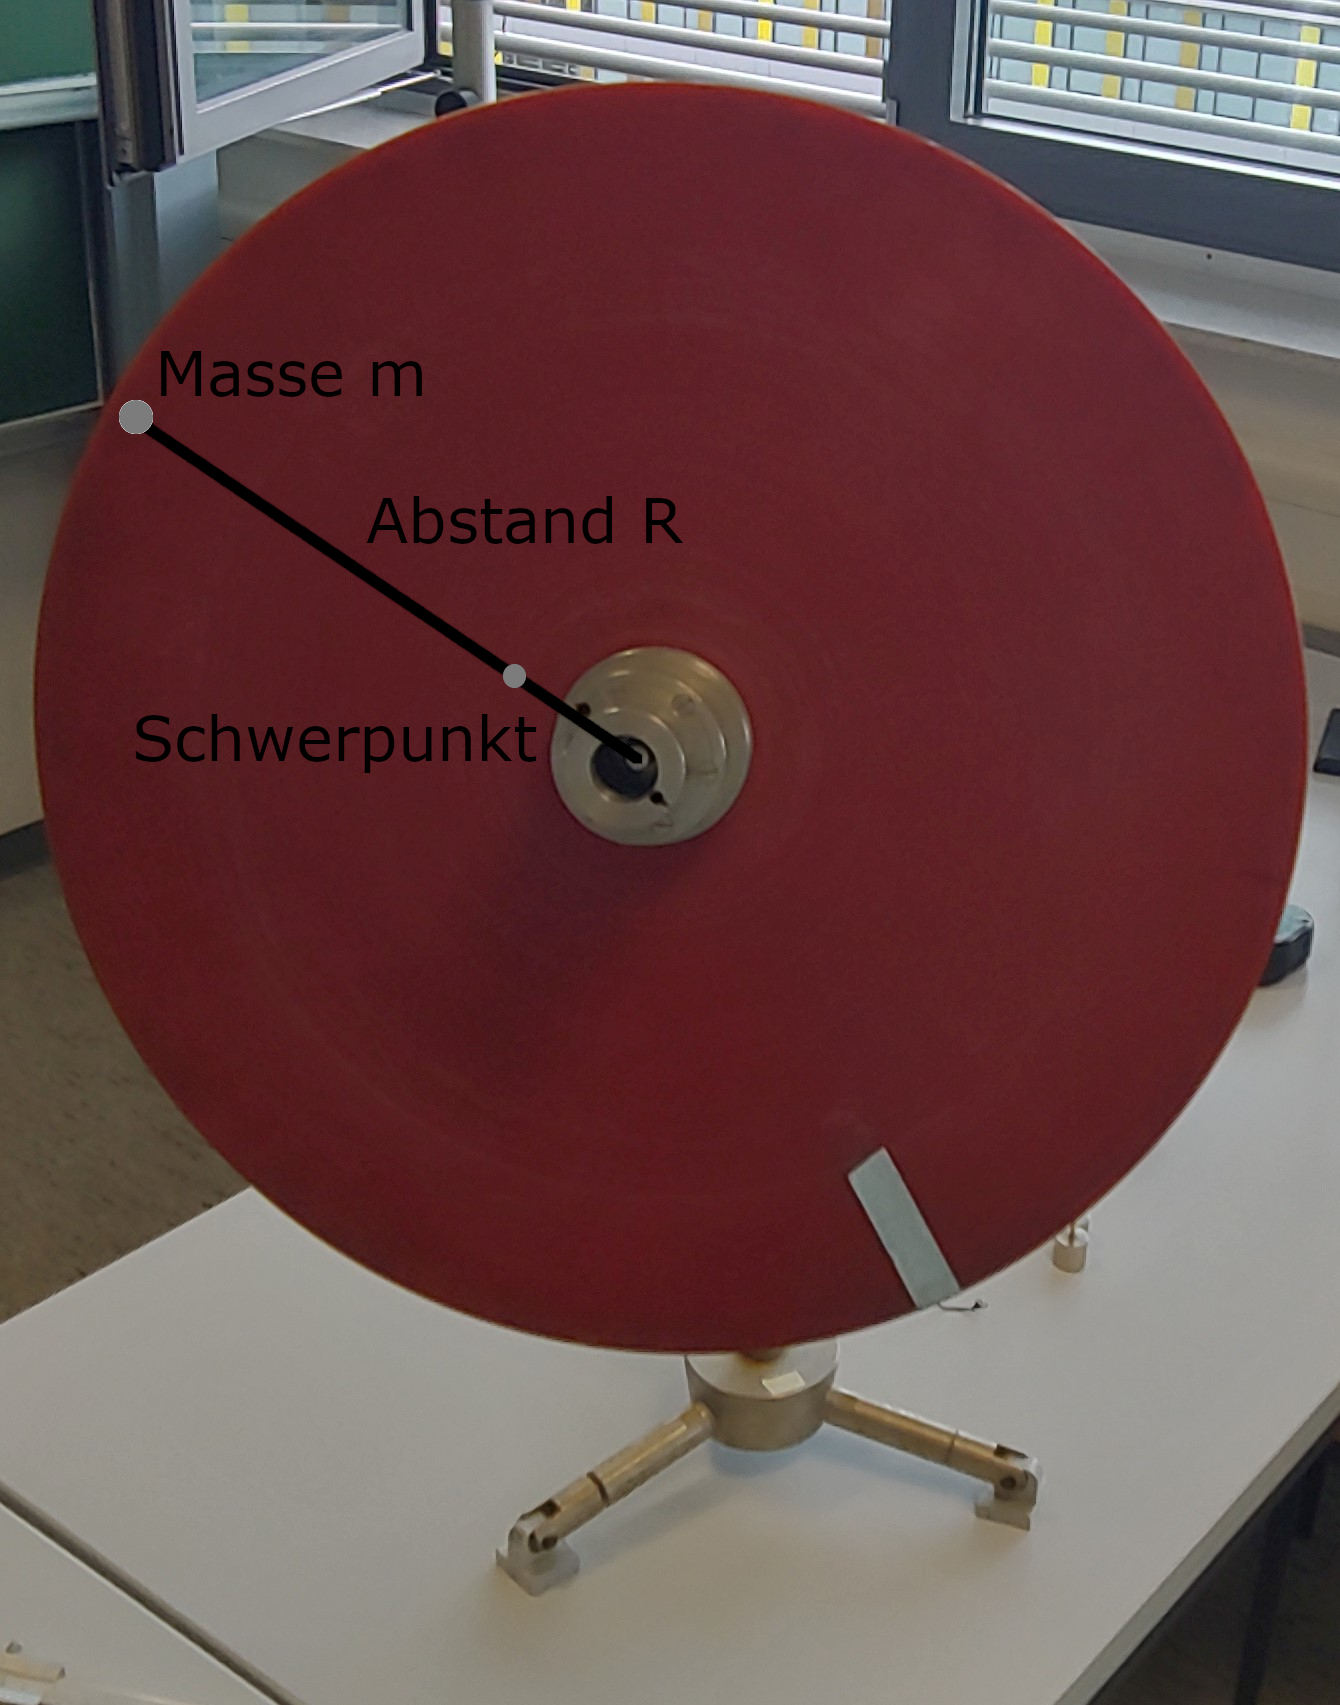
\includegraphics[width=0.5\textwidth]{schwingung_aufbau.png}
		\caption{\label{fig:Schwingung_Aufbau}Der Versuchsaufbau mit relevanten Größen}
	\end{figure}

	\subsection{Messergebnisse}
	Das Gewicht das außen an der Scheibe angebracht wird, wurde mit Hilfe einer Waage auf \(\SI{101}{\gram}\) bestimmt.
	Die benutzte Waage hat eine Genauigkeit von einem Gramm.
	Der Abstand \(R\) (Siehe Abbildung~\ref{fig:Schwingung_Aufbau}) vom Mittelpunkt der Scheibe
	bis zum angehängten Gewicht beträgt \(\SI{18,7}{cm}\).
	Das dazu verwendete Maßband hat eine Genauigkeit von einem Millimeter. \\
	Die Schwingungsdauer wurde für zehn Perioden mit \(\SI{32,04}{\second}\) gemessen.
	Die Handystoppuhr die für die Zeitmessung verwendet wurde hat eine Genauigkeit von einer Millisekunde. <- Centisekunde

	\subsection{Auswertung}

	\subsubsection{Formeln}
	Das Trägheitsmoment der Scheibe, \(I\) wird durch anbringen der Masse \(m\) verändert.
	Das Trägheits\-moment \(I\) bezieht sich auf die Achse die durch den Mittelpunkt und Schwerpunkt der Scheibe geht.
	Die kleine Masse verschiebt den Schwerpunkt nach außen (Siehe~\ref{fig:Schwingung_Aufbau}).
	Das neue Trägheitsmoment von Scheibe und Masse gemeinsam nennen wir \(I'\). Dieses können wir mit dem Steiner'schen Satz berechnen (Quelle~\cite{ExPhy1}).
	\begin{equation}\label{eq:Neues_Trägheismoment}
		I' = I + m \cdot R^2
	\end{equation}
	Wie wir bereits im Kapitel~\ref{Allgemeine_Theorie} in Gleichung~(\ref{eq:trägheitsmoment_diskret}) gesehen haben, steuert eine weitere diskrete Masse den Anteil \( m_i r_i^2\)
	zum Trägheitsmoment dazu. Hier \( m \cdot R^2\).
	Das Trägheitsmoment \(I'\) ist zur Achse des Drehmoments \(I\) parallel nach außen, in Richtung der kleinen Masse, verschoben.
	Die Achse des Trägheitsmoments \(I'\) geht jedoch nicht durch den neuen Schwerpunkt, da sonst das System nicht schwingen würde. \\ % TODO: ???
	Da die Achse nun nicht mehr durch den Schwerpunkt geht, gibt es ein Direktionsmoment. Es hat die selbe physikalische Bedeutung wie die rücktreibenden Kraft beim Federpendel.
	Das durch die Masse erzeugte Drehmoment ist: \(M = R \times \vec{F}\), da wir aber nur mit Beträgen rechnen folgt:
	\begin{equation}
		|\vec{M}| = M = R \cdot F \cdot \sin \varphi
	\end{equation}
	Die Kraft ist hier die Gewichtskraft der kleinen Masse also \(F = m \cdot g\). Zusammen:
	\begin{equation}
		M = R \cdot m \cdot g \cdot \sin \varphi
	\end{equation}
	Das Direktionsmoment ist definiert als \(D = \frac{M}{\varphi}\), also rücktreibendes Drehmoment pro Winkeleinheit:
	\begin{equation}
		D = \frac{M}{\varphi} = \frac{ R \cdot m \cdot g \cdot \sin \varphi }{ \varphi }
	\end{equation}
	Lenken wir nur kleine Winkel aus können wir für das Direktionsmoment die Kleinwinkelnäherung (Taylorentwicklung von \( \sin \varphi \) abgebrochen nach der ersten Ordnung)
	anwenden. Wir ersetzen also \( \sin \varphi \) mit \( \varphi \). Im Experiment wurde auf Grund dieser Näherung die Scheibe nur um einen kleinen Winkel ausgelenkt.
	\begin{equation}\label{eq:Genähertes_Direktionsmoment}
		D = \frac{ R \cdot m \cdot g \cdot \sin \varphi }{ \varphi } \approx \frac{ R \cdot m \cdot g \cdot \varphi }{ \varphi } = R \cdot m \cdot g
	\end{equation}
	% TODO: Aufstellen DGL mit MMdP Skript Seite 109
	Für ein Pendel mit Direktionsmoment gilt für die Schwingungsdauer:
	\begin{equation}
		T = 2 \pi \sqrt{ \frac{I'}{D} }
	\end{equation}
	Setzen wir für \(I'\) und \(D\) die in den Formeln (\ref{eq:Neues_Trägheismoment}) und (\ref{eq:Genähertes_Direktionsmoment}) gegebenen Beziehungen ein, erhalten wir die folgende Formel:
	\begin{equation}
		T = 2 \pi \sqrt{ \frac{ I + m \cdot R^2 }{ R \cdot m \cdot g } }
	\end{equation}
	Im letzten Schritt formen wir die Gleichung nach dem zu bestimmenden Trägheitsmoment \(I\) um:
	\begin{equation}
		\begin{gathered} \label{eq:Trägheitsmoment_Schwingung}
			T = 2 \pi \sqrt{ \frac{ I + m \cdot R^2 }{ m \cdot g \cdot R } } \Leftrightarrow \\
			\frac{T}{ 2 \pi } = \sqrt{ \frac{ I + m \cdot R^2 }{ m \cdot g \cdot R } } \Leftrightarrow \\
			{\left( \frac{T}{ 2 \pi } \right)}^2 = \frac{ I + m \cdot R^2 }{ m \cdot g \cdot R } \Leftrightarrow \\
			\frac{T^2}{4 \pi^2} \cdot m \cdot g \cdot R = I + m \cdot R^2 \Leftrightarrow \\
			\frac{T^2}{4 \pi^2} \cdot m \cdot g \cdot R - m \cdot R^2 = I \Leftrightarrow \\
			I = R \cdot m \cdot \left( \frac{T^2 \cdot g }{ 4 \pi^2 } - R \right)
		\end{gathered}
	\end{equation}
	Einheitenkontrolle:
	\begin{equation}
		[I] = \unit{\metre} \cdot \unit{\kilogram} \cdot \left( \unit{\second^2} \cdot \unit{\frac{\metre}{\second^2}} - \unit{\metre} \right) = \unit{\kilogram \cdot \metre^2}
	\end{equation}

	\subsubsection{Trägheitsmomentberechnung}
	Gemessen wurden im Experiment zehn Periodendauern. Da bei einer harmonischen Schwingung die Periodendauer nicht von der Auslenkung abhängt und hier also konstant ist, teilen wir unseren gemessenen Wert durch zehn:
	\begin{equation}
		T = \frac{ \SI{32,04}{\second} }{ 10 } = \SI{3,204}{\second}
	\end{equation}
	Zur Berechnung des Ergebnisses setzen wir die Erdbeschleunigung \(\SI{9,81}{\frac{\metre}{\second^2}}\), die kleine Masse \(m = \SI{101}{\gram} = \SI{0,101}{\kilogram} \),
	den Abstand \(R = \SI{18,7}{cm} = \SI{0,187}{\metre} \), sowie die Periodendauer \( T = \SI{3,204}{\second} \) in Formel (\ref{eq:Trägheitsmoment_Schwingung}) ein:
	\begin{equation}
		I = \SI{0,187}{\metre} \cdot \SI{0,101}{\kilogram} \cdot \left( \frac{ {( \SI{3,204}{\second} )}^2 \cdot \SI{9,81}{\frac{\metre}{\second^2}} }{ 4 \pi^2 } - \SI{0,187}{\metre} \right) = \SI{0,0446}{\kilogram \cdot \metre^2}
	\end{equation}
	% 0.187 metre * 0.101 kilogram * ( ((3.203 seconds)^2 * 9.81 metres per second squared )/(4 pi^2) - 0.187 metre)

	\subsubsection{Fehlerrechnung}
	Wie in Teilversuch 1 berechnen wir den maximalen Fehler:
	\begin{equation}
		\Delta I =
		\left| \frac{\partial I}{\partial m} \right| \Delta m +
		\left| \frac{\partial I}{\partial R} \right| \Delta R +
		\left| \frac{\partial I}{\partial T} \right| \Delta T
	\end{equation}
	Dazu berechnen wir die partiellen Ableitungen von Gleichung (\ref{eq:Trägheitsmoment_Schwingung}):
	\begin{equation}
		\begin{aligned}
			\frac{\partial I}{\partial m} & = \frac{\partial}{\partial m} \left( \frac{T^2}{4 \pi^2} \cdot m \cdot g \cdot R - m R^2 \right) = \frac{T^2}{4 \pi^2} \cdot g \cdot R - R^2                                                              \\
			\frac{\partial I}{\partial R} & = \frac{\partial}{\partial R} \left( \frac{T^2}{4 \pi^2} \cdot m \cdot g \cdot R - m R^2 \right) = \frac{T^2}{4 \pi^2} \cdot m \cdot g - 2 m R = m \cdot \left( \frac{T^2 \cdot g }{4 \pi^2} - 2R \right) \\
			\frac{\partial I}{\partial T} & = \frac{\partial}{\partial T} \left( \frac{T^2}{4 \pi^2} \cdot m \cdot g \cdot R - m R^2 \right) = \frac{T}{2 \pi^2} \cdot m \cdot g \cdot R  = \frac{T \cdot m \cdot g \cdot R}{2 \pi^2 }                \\
		\end{aligned}
	\end{equation}
	Wir setzen die partiellen Ableitungen in die Formel für den maximalen Fehler ein:
	\begin{equation}\label{eq:Maximaler_Fehler_Schwingung}
		\Delta I =
		\left| \frac{T^2}{4 \pi^2} \cdot g \cdot R - R^2 \right| \Delta m +
		\left| m \cdot \left( \frac{T^2 \cdot g }{4 \pi^2} - 2R \right) \right| \Delta R +
		\left| \frac{T \cdot m \cdot g \cdot R}{2 \pi^2 } \right| \Delta T
	\end{equation}
	Der Fehler der Abstandsmessung \(\Delta R\) wäre allein vom Maßband \(\SI{1}{mm}\).
	Wegen des Zylindrischen Ansatzes auf der Vorderseite der Scheibe lässt sich der Abstand aber mitnichten so genau messen.
	Wir setzen hier einen Fehler von \(\SI{5}{mm} = \SI{0,005}{\metre} \) an. \\
	Der Messfehler der Waage ist \(\Delta m = \SI{1}{\gram}\). \\
	Die Auflösung der für den Versuch verwendeten Stoppuhr (Handystoppuhr) ist eine \(\SI{1}{ms}\).
	Die menschliche Reaktionszeit beträgt aber bereits \(\approx \SI{180}{ms} \) (Siehe~\cite{Reaktionszeit})
	Gestoppt wurde am Umkehrpunkt der Pendelschwingung, wobei diese mit bloßem Auge beobachtet wurde, was das Ergebnis weiter verfälscht.
	Bis dann die Stoppuhr gedrückt wurde sind bereits \(\approx \SI{0,2}{\second}\) vergangen.
	Da die gleiche Verzögerung auch beim Beginn der Messung entsteht, schätzen wir den Messfehler auf \(\SI{0,25}{\second}\).
	Deutlich genauere Messwerte wären mit Hilfe von Videoanalyse zu bekommen, wobei der Messfehler hier die Framerate des Videos wäre.
	Der Messfehler bezieht sich aber auf zehn Periodendauern weshalb wir die Unsicherheit hier noch einmal durch zehn teilen:
	\begin{equation}
		\Delta T = \frac{\SI{0,25}{\second}}{10} = \SI{0,025}{\second}
	\end{equation}
	Wir setzen nun die Messfehler \( \Delta m = \SI{0,001}{\kilogram} \), \( \Delta R = \SI{0,005}{\metre} \) und \(\Delta T = \SI{0,025}{\second} \), sowie alle weiteren gemessenen Größen und Variablen
	\(g = \SI{9,81}{\frac{\metre}{\second^2}} \), \(m = \SI{0,101}{\kilogram} \), \(R = \SI{0,187}{\metre} \) und \( T = \SI{3,204}{\second} \) in Gleichung~(\ref{eq:Maximaler_Fehler_Schwingung}) ein:
	\begin{equation}
		\begin{aligned}
			\Delta I & =                                                                                                                                                                                                     \\
			         & \left| \frac{ {\SI{3,204}{\second}}^2 }{4 \pi^2} \cdot \SI{9,81}{\frac{\metre}{\second^2}} \cdot \SI{0,187}{\metre} - {\left(\SI{0,187}{\metre}\right)}^2 \right| \cdot \SI{0,001}{\kilogram} +       \\
			         & \left| \SI{0,101}{\kilogram} \cdot \left( \frac{ {\SI{3,204}{\second}}^2 \cdot \SI{9,81}{\frac{\metre}{\second^2}} }{4 \pi^2} - 2 \cdot \SI{0,187}{\metre} \right) \right| \cdot \SI{0,005}{\metre} + \\
			         & \left| \frac{ \SI{3,204}{\second} \cdot \SI{0,101}{\kilogram} \cdot \SI{9,81}{\frac{\metre}{\second^2}} \cdot \SI{0,187}{\metre} }{2 \pi^2 } \right| \cdot \SI{0,025}{\second}                        \\
			         & = \SI{0.002293}{ \kilogram \cdot \metre^2 }
		\end{aligned}
	\end{equation}
	% abs((3.204s)^2/(4*pi^2)*9.81m/s^2 *0.187m - (0.187m)^2 ) * 0.001kg + abs( 0.101kg * ((3.204s)^2 * 9.81m/s^2 /(4*pi^2) - 2*0.187 m)) * 0.005m + abs((3.204s*0.101kg* 9.81m/s^2* 0.187m)/(2*pi^2))*0.025s
	In diesem maximalen Fehler bleibt die Kleinwinkelnäherung unberücksichtigt etc.

	\subsubsection{Endergebnis}
	Das Trägheitsmoment beträgt bei der Bestimmung über eine Pendelbewegung also:
	\begin{equation}
		I = \SI{4,46e-2}{ \kilogram \cdot \metre^2 } \pm \SI{0,229e-2}{ \kilogram \cdot \metre^2 }
	\end{equation}

	\section{Bestimmung über Präzessionsbewegung}

	\subsection{Durchführung}
	\subsubsection{Materialien}
	\begin{itemize}
		\item Kreisel (siehe allgemeiner Aufbau)
		\item Gewicht
		\item Schnur
		\item Waage
		\item Stoppuhr (Handy)
		\item Handzähler (Klicker)
		\item Maßband
	\end{itemize}
	Um das Trägheitsmoment mit Hilfe einer Präzessionsbewegung zu bestimmen muss zuerst eine solche Bewegung hervorgerufen werden.
	Dazu wird, wie in Abbildung~\ref{fig:Präzession} zu sehen das Gewicht an den Kreisel gehängt, dessen Masse \(m\) zuvor mit der Waage bestimmt wurde (das Gewicht der Schnur wird dabei mitgewogen).\\
	Nun wird der Kreisel in einer waagerechten Position gehalten und die Scheibe wird in Rotation versetzt.
	Dann wird der Kreisel losgelassen und die Präzessionsbewegung setzt ein.
	Nun stoppt eine Person die Zeit \(T\), welche ein Umlauf der Präzession benötigt, während eine andere Person die Umdrehungen der Scheibe \(n\) in dieser Zeit mit dem Handzähler zählt.\\
	Dies wird zehn mal wiederholt, wobei die Winkelgeschwindigkeit der Scheibe und die angehängte Masse variiert werden.\\
	Zudem wird mit dem Maßband der Abstand \(s\) des angehängten Gewichts von der Achse, um welche die Präzession stattfindet, gemessen (Abbildung~\ref{fig:Präzession})
	\begin{figure}
		\centering
		\includegraphics[width=1\textwidth]{PräzessionEdit.jpg}
		\caption{\label{fig:Präzession}Aufbau zur Präzession}
	\end{figure}

	\subsection{Messergebnisse}
	Der Abstand \(s\) wurde auf \(s = \SI{26,9}{cm} \) bestimmt, die restlichen Messwerte und \( \frac{mT^2}{n} \) werden in eine Tabelle eingetragen:
	\begin{center}\label{tab:MesswertePräzession}
		\begin{tabular}{ |c|c|c|c| }
			\hline
			\(m[\unit{\gram}]\) & \(T[\unit{\second}]\) & \(n\) & \( \frac{mT^2}{n}[\unit{\kilogram \cdot \second^2}] \) \\
			\hline
			202                 & 12,97                 & 33    & 1,03 \\
			202                 & 10,61                 & 20    & 1,14 \\
			202                 & 12,70                 & 38    & 0,86 \\
			202                 & 11,09                 & 25    & 0,99 \\
			202                 & 10,83                 & 23    & 1,03 \\
			99                  & 18,27                 & 37    & 0,89 \\
			99                  & 17,28                 & 34    & 0,87 \\
			99                  & 20,58                 & 51    & 0,82 \\
			99                  & 15,71                 & 21    & 1,16 \\
			99                  & 22,21                 & 64    & 0,76 \\
			\hline
		\end{tabular}
	\end{center}
	Den Fehler der Längenmessung schätzen wir auf \( \Delta s = \SI{2}{mm} \), etwas größer als die naheliegenden Genauigkeit des Maßbands \(\SI{1}{mm}\),
	da das Maßband sich nicht perfekt an die zu messende Strecke anlegen ließ

	\subsection{Auswertung}
	\subsubsection{Formeln}
	Wenn sich ein symmetrischer Kreisel in einer Rotationsbewegung befindet und ein Drehmoment senkrecht an seiner Drehachse angreift, dann wirkt ein resultierendes Drehmoment \( \vec M\) senkrecht zur Drehachse und dem angreifenden Moment.
	Da \( \vec M = \vec{\dot L} \) gilt (analog zu \(\vec F = \vec{\dot p}\) bei Translationsbewegungen), ist also die Änderung von \(\vec L\) senkrecht zu \(\vec L\).
	Daher muss der Betrag von \( \vec L \) konstant bleiben, und \( \vec L \) kann nur eine gleichmäßige Drehbewegung beschreiben (so wie bei Kreisbewegungen \(\vec a = \vec{\dot v}\) senkrecht auf \(\vec v\) steht). Da der Drehimpuls senkrecht auf der Drehscheibe steht führt die Achse, an welcher die Scheibe angebracht ist, eine Drehbewegung aus.\\ % TODO: Verstehe ich nicht. Ließ vielleicht selber nochmal drüber :)
	%
	Diese Präzessionsbewegung hat eine Winkelgeschwindigkeit \( \omega_p \), welche sich bestimmen lässt, indem man die senkrechte Änderung \( d\vec L \) von \( \vec L \) in der Zeit \( dt \) betrachtet:
	\begin{equation}
		d\vec L = \vec M \, d t
	\end{equation}
	Dadurch dreht sich \( \vec L \) um den Winkel \( d \varphi \):
	\begin{equation}
		d \varphi = \frac{ dL }{ L \cdot \sin(\alpha) } = \frac{ Mdt }{ L \cdot \sin(\alpha) }
	\end{equation}
    Wobei \(\alpha\) der Winkel zwischen der Symmetrieachse des Kegels, den \(\vec L\) beschreibt, und \(\vec L\) selbst ist. Und \(dL\) ist ein Kreisbogen der Grundfläche des Kegels, \( L \cdot \sin(\alpha) \) ist also der Radius der Grundfläche. Da die Länge des Kreisbogens (wenn man mit dem Bogenmaß rechnet) gleich dem Radius des Kreises mal dem Winkel \(d\varphi\) ist, gilt die Gleichung.
	Es ergibt sich also für die Präzessionsfrequenz \( \omega_p \):
	\begin{equation}\label{eq:omegap}
		\omega_p = \frac{ d\varphi }{ dt } = \frac{ M }{ L \cdot \sin(\alpha) }
	\end{equation}
	In unserem Experiment wird das Drehmoment \(M\) durch die Schwerkraft hervorgerufen. Das angreifende Drehmoment hängt damit von der Neigung der präzedierenden Achse ab (Die Achse, an welcher die Drehscheibe befestigt ist).
	Wenn die Achse horizontal liegt, ist der Betrag des Drehmoments gegeben als \(M = mgs\), wenn die Achse schief ist, muss die senkrechte Komponente betrachtet werden (senkrecht zu der Achse, an welcher die Scheibe montiert ist).
	Diese Komponente erhält man, indem man das Drehmoment für den horizontalen Fall mit dem Kosinus des Winkels zwischen dem gesuchten senkrechten Drehmoment und dem für den horizontalen Fall multipliziert. 
	Dieser Winkel ist gegeben als \(90^{\circ} - \alpha\), und es ergibt sich:
	\begin{equation}
		M = m g s \cdot \sin(\alpha)
	\end{equation}
	Dadurch ist \( \omega_p \) unabhängig davon, wie stark die Achse geneigt ist (\(M\) in Gleichung~\ref{eq:omegap} einsetzen):
	\begin{equation}
		\omega_p = \frac{ m g s }{L} = \frac{ m g s }{ I \omega}
	\end{equation}
	Umgestellt nach dem gesuchten Trägheitsmoment \(I\):
	\begin{equation}
		I = \frac{ m g s }{\omega_p \omega}
	\end{equation}
	(Nach Kapitel 2.4 \textit{Der Kreisel} aus Quelle~\cite{Gerthsen}) \\
	Nun ergibt mit \( \omega_p = \frac{ 2 \pi }{ T } \) und \( \omega = \frac{2 \pi n}{ T } \) (Aus~\cite{AnleitungPraktikum}):
	\begin{equation}\label{eq:IPräzession}
		I = m g s \frac{T}{2 \pi} \frac{T}{2 \pi n} = \frac{g \cdot s}{ 4 \pi^2 } \frac{ m T^2 }{ n }
	\end{equation}

	\subsubsection{Bestimmung des Trägheitsmoments}
	Aus den Messwerten aus~\ref{tab:MesswertePräzession} ergibt sich für \( \frac{mT^2}{n} \) ein Mittelwert von:
	\begin{equation}
		\overline{ \left( \frac{ m T^2 }{n} \right) } = \SI{0,955}{\kilogram \cdot \second^2}
	\end{equation}
	Um das Trägheitsmoment zu berechnen setzen wir \(g = \SI{9,81}{ \frac{\metre}{\second^2} } \), \(s = \SI{0,269}{\metre} \)
	und den oben berechneten Mittelwert für \( \frac{ m T^2 }{n} = \SI{0,955}{\kilogram \cdot \second^2} \) in Gleichung (\ref{eq:IPräzession}) ein:
	\begin{equation}
		I = \frac{ \SI{9,81}{ \frac{\metre}{\second^2} } \cdot \SI{0,269}{\metre} \cdot \SI{0,955}{\kilogram \cdot \second^2} }{ 4 \pi^2 } = \SI{6,4e-2}{\kilogram \cdot \metre^2}
	\end{equation}

	\subsubsection{Fehlerrechnung}
	Der Maximahlfehler von \( I \) ist gegeben als:
	\begin{equation}
		\Delta I = \left| \frac{\partial I}{\partial s} \right| \Delta s
		+ \left| \frac{\partial I}{\partial \frac{mT^2}{n}} \right| \Delta \left( \frac{mT^2}{n} \right)
	\end{equation}
	Dazu berechnen wir die beiden partiellen Ableitungen von Gleichung~(\ref{eq:IPräzession})
	\begin{equation}
		\begin{gathered}
			\frac{\partial I}{\partial s}  = \frac{\partial}{\partial s} \frac{g \cdot s}{ 4 \pi^2 } \frac{ m T^2 }{ n } = \frac{g}{ 4 \pi^2 } \frac{ m T^2 }{ n } \\
			\frac{\partial I}{\partial \frac{mT^2}{n}} = \frac{\partial}{\partial \frac{mT^2}{n}} = \frac{g \cdot s}{ 4 \pi^2 } \frac{ m T^2 }{ n } = \frac{g \cdot s}{ 4 \pi^2 }
		\end{gathered}
	\end{equation}
	Eingesetzt:
	\begin{equation}
		\frac{g}{4 \cdot \pi^2} \cdot \frac{m \cdot T^2 }{n} \Delta s + \frac{ g \cdot s }{4 \cdot \pi^2} \Delta \left( \frac{ m T^2 }{n} \right)
	\end{equation}
	Einheitenrechnung
	\begin{equation}
		\begin{gathered}
			\left( \unit{\frac{\metre}{\second^2}} \cdot \unit{\kilogram} \cdot \unit{\second^2} \right) \cdot \unit{\metre} +
			\left( \unit{\frac{\metre}{\second^2}} \cdot \unit{\metre} \right) \cdot \left( \unit{\kilogram} \cdot \unit{\second^2} \right) = \\
			\unit{\metre \cdot \kilogram} \cdot \unit{\metre} + \unit{\frac{\metre^2}{\second^2}} \cdot \unit{\kilogram \cdot \second^2} = \unit{\kilogram \cdot \metre^2}
		\end{gathered}
	\end{equation}
	Der Fehler von \( \frac{ m T^2 }{n} \) nehmen wir so groß an wie die größte Abweichung eines Wertes vom Mittelwert. \\
	Der Wert \( \SI{1,16}{\kilogram \cdot \second^2}\) weicht am stärksten vom Mittelwert \( \SI{0,955}{\kilogram \cdot \second^2} \) ab, damit berechnen wir den Maximalfehler von \( \frac{ m T^2 }{ n } \) auf:
	\begin{equation}
		\Delta \left( \frac{mT^2}{n} \right) = \SI{1,16}{\kilogram \cdot \second^2} - \SI{0,955}{\kilogram \cdot \second^2} = \SI{0,205}{\kilogram \cdot \second^2}
	\end{equation}
	Den Fehler der Längenmessung schätzen wir auf \( \Delta s = \SI{2}{mm} \), etwas größer als die naheliegenden Genauigkeit des Maßbands \(\SI{1}{mm}\),
	da das Maßband sich nicht perfekt an die zu messende Strecke anlegen ließ. Der maximale Fehler von \( I \) liegt damit bei: % TODO:Werte?
	\begin{equation}
		\Delta I = \left( \frac{ \SI{9,81}{ \frac{\metre}{\second^2} } }{ 4 \pi^2 } \cdot \SI{0,955}{\kilogram \cdot \second^2} \right) \cdot \SI{0,002}{\metre} +
		\frac{ \SI{9,81}{ \frac{\metre}{\second^2} } \cdot \SI{0,269}{\metre} }{ 4 \pi^2 } \cdot \SI{0,205}{\kilogram \cdot \second^2} = \SI{0,0142}{\kilogram \cdot \metre^2}
	\end{equation}

	\subsubsection{Endergebnis}
	Für das Trägheitsmoment ergibt sich bei der Bestimmung über eine Präzessionsbewegung also:
	\begin{equation}
		I = \SI{6,4e-2}{\kilogram \cdot \metre^2} \pm \SI{1,42e-2}{\kilogram \cdot \metre^2}
	\end{equation}

	\section{Fazit}
	Die drei Trägheitsmomente der drei Teilversuche sind nun also:
	\begin{equation*}
		\begin{aligned}
			I_1 & = \SI{4,87e-2}{ \kilogram \cdot \metre^2 } & \pm \SI{0,15e-2}{ \kilogram \cdot \metre^2 } \\
			I_2 & = \SI{4,46e-2}{ \kilogram \cdot \metre^2 } & \pm \SI{0,23e-2}{ \kilogram \cdot \metre^2 } \\
			I_3 & = \SI{6,40e-2}{ \kilogram \cdot \metre^2 } & \pm \SI{1,42e-2}{\kilogram \cdot \metre^2}
		\end{aligned}
	\end{equation*}
	Wir sehen, dass trotz der graphischen Auswertung Teilversuch 1 den kleinsten Fehler hat. Die Fehler für Teilversuche 1 und 2 sind im Vergleich zu Teilversuch 3
	relativ klein. Auch das berechnete Trägheitsmoment in Versuch 3 ist weicht bedeutend von den anderen beiden ab.
	Der Versuch über die Bestimmung mit Hilfe der Präzession hatte mit Abstand das meiste Potential für Messfehler und hatte auch einige in der Fehlerrechnung unberücksichtigte Fehlerquellen.
	Die Messungen mit dem Handzähler sind, da sich die Kreisscheibe sehr schnell dreht wahrscheinlich immer um 2 - 3 Umdrehungen falsch. Außerdem hat hier die Reibung der sich drehenden Scheibe den
	größten Einfluss. Während des Versuch konnten wir bereits beobachten das sich die Scheibe zum Ende einer Rotation bereits deutlich langsamer drehte.
	Dieser Versuch ist damit wohl der schlechteste Versuch, ungenauste Messmethode.

	Die beiden ersten Versuche sind relativ simpel. Bei dem ersten handelt es sich nur um eine beschleunigte Bewegung, beim zweiten um eine Schwingung, deswegen
	sind ihre Fehler erwartbarer Weise klein.

	Der Theoriefehler mit der Kleinwinkelnäherung in Versuch 2 fällt, dank der Messvorkehrungen und der allgemeinen Güte dieser Näherung hier nicht ins Gewicht.
	Erstaunt waren wir auch bei der graphischen Auswertung von Versuch 1, weil die Messwerte erstaunlich genau auf der vorhergesagten Gerade lagen,
	dennoch wird der Punkt (0, 0) hier nicht mit einbezogen der überhaupt nicht auf der Gerade liegt aber natürlich, da die Scheibe zum Start des Experiments keine Winkelauslenkung hatte.

	Der reale Wert des Trägheitsmoments liegt wohl zwischen den in Versuch 1 und 2 bestimmten Werten.

	Um einschätzen zu können ob die berechneten Ergebnisse die richtige Größenordnung haben, bedienen wir uns einer weiteren Methode zur Bestimmung des Drehmoments.
	Alternativ hätte man den Radius und das Gewicht der Scheibe messen können und daraus, mit der Formel \( I = \frac{1}{2} m \cdot r^2 \)(Siehe Trägheitsmoment einer Scheibe im Buch Halliday Physik~\cite{HallidayPhysik}).
	Wir berechnen nun aus dem Ergebnis des ersten Versuchs, sowie der Messung des zweiten Versuchs (fast eine Radiusmessung) ein Gewicht für die Scheibe. TODO: Sinnvoll?

	TODO: Welcher Versuch ist am Besten geeignet, am einfachsten, am genausten, etc. \ldots um das Trägheitsmoment zu bestimmen.
	Vergleich der Ergebnisse
	Diskutiere z.B Reibungseffekte, Kleinwinkelnäherung, etc.
	Fazit beste Methode, z.B. kleinster Fehler, Durchführung am wenigsten Aufpassen.
	Direkt bestimmen mit Gewicht und Radius
	Masse raten/bestimmen aus Trägheitsmomenten
	Trägheitsmoment in Relation setzen
	Fehler Graphische Auswertung 1 nicht 0,0.
	Versuch 1 graphische Auswertung, nicht rein mathematisch

	\printbibliography[title={Quellen}]

	\begin{figure}[!ht]\label{fig:Messwerte1}
		\centering
		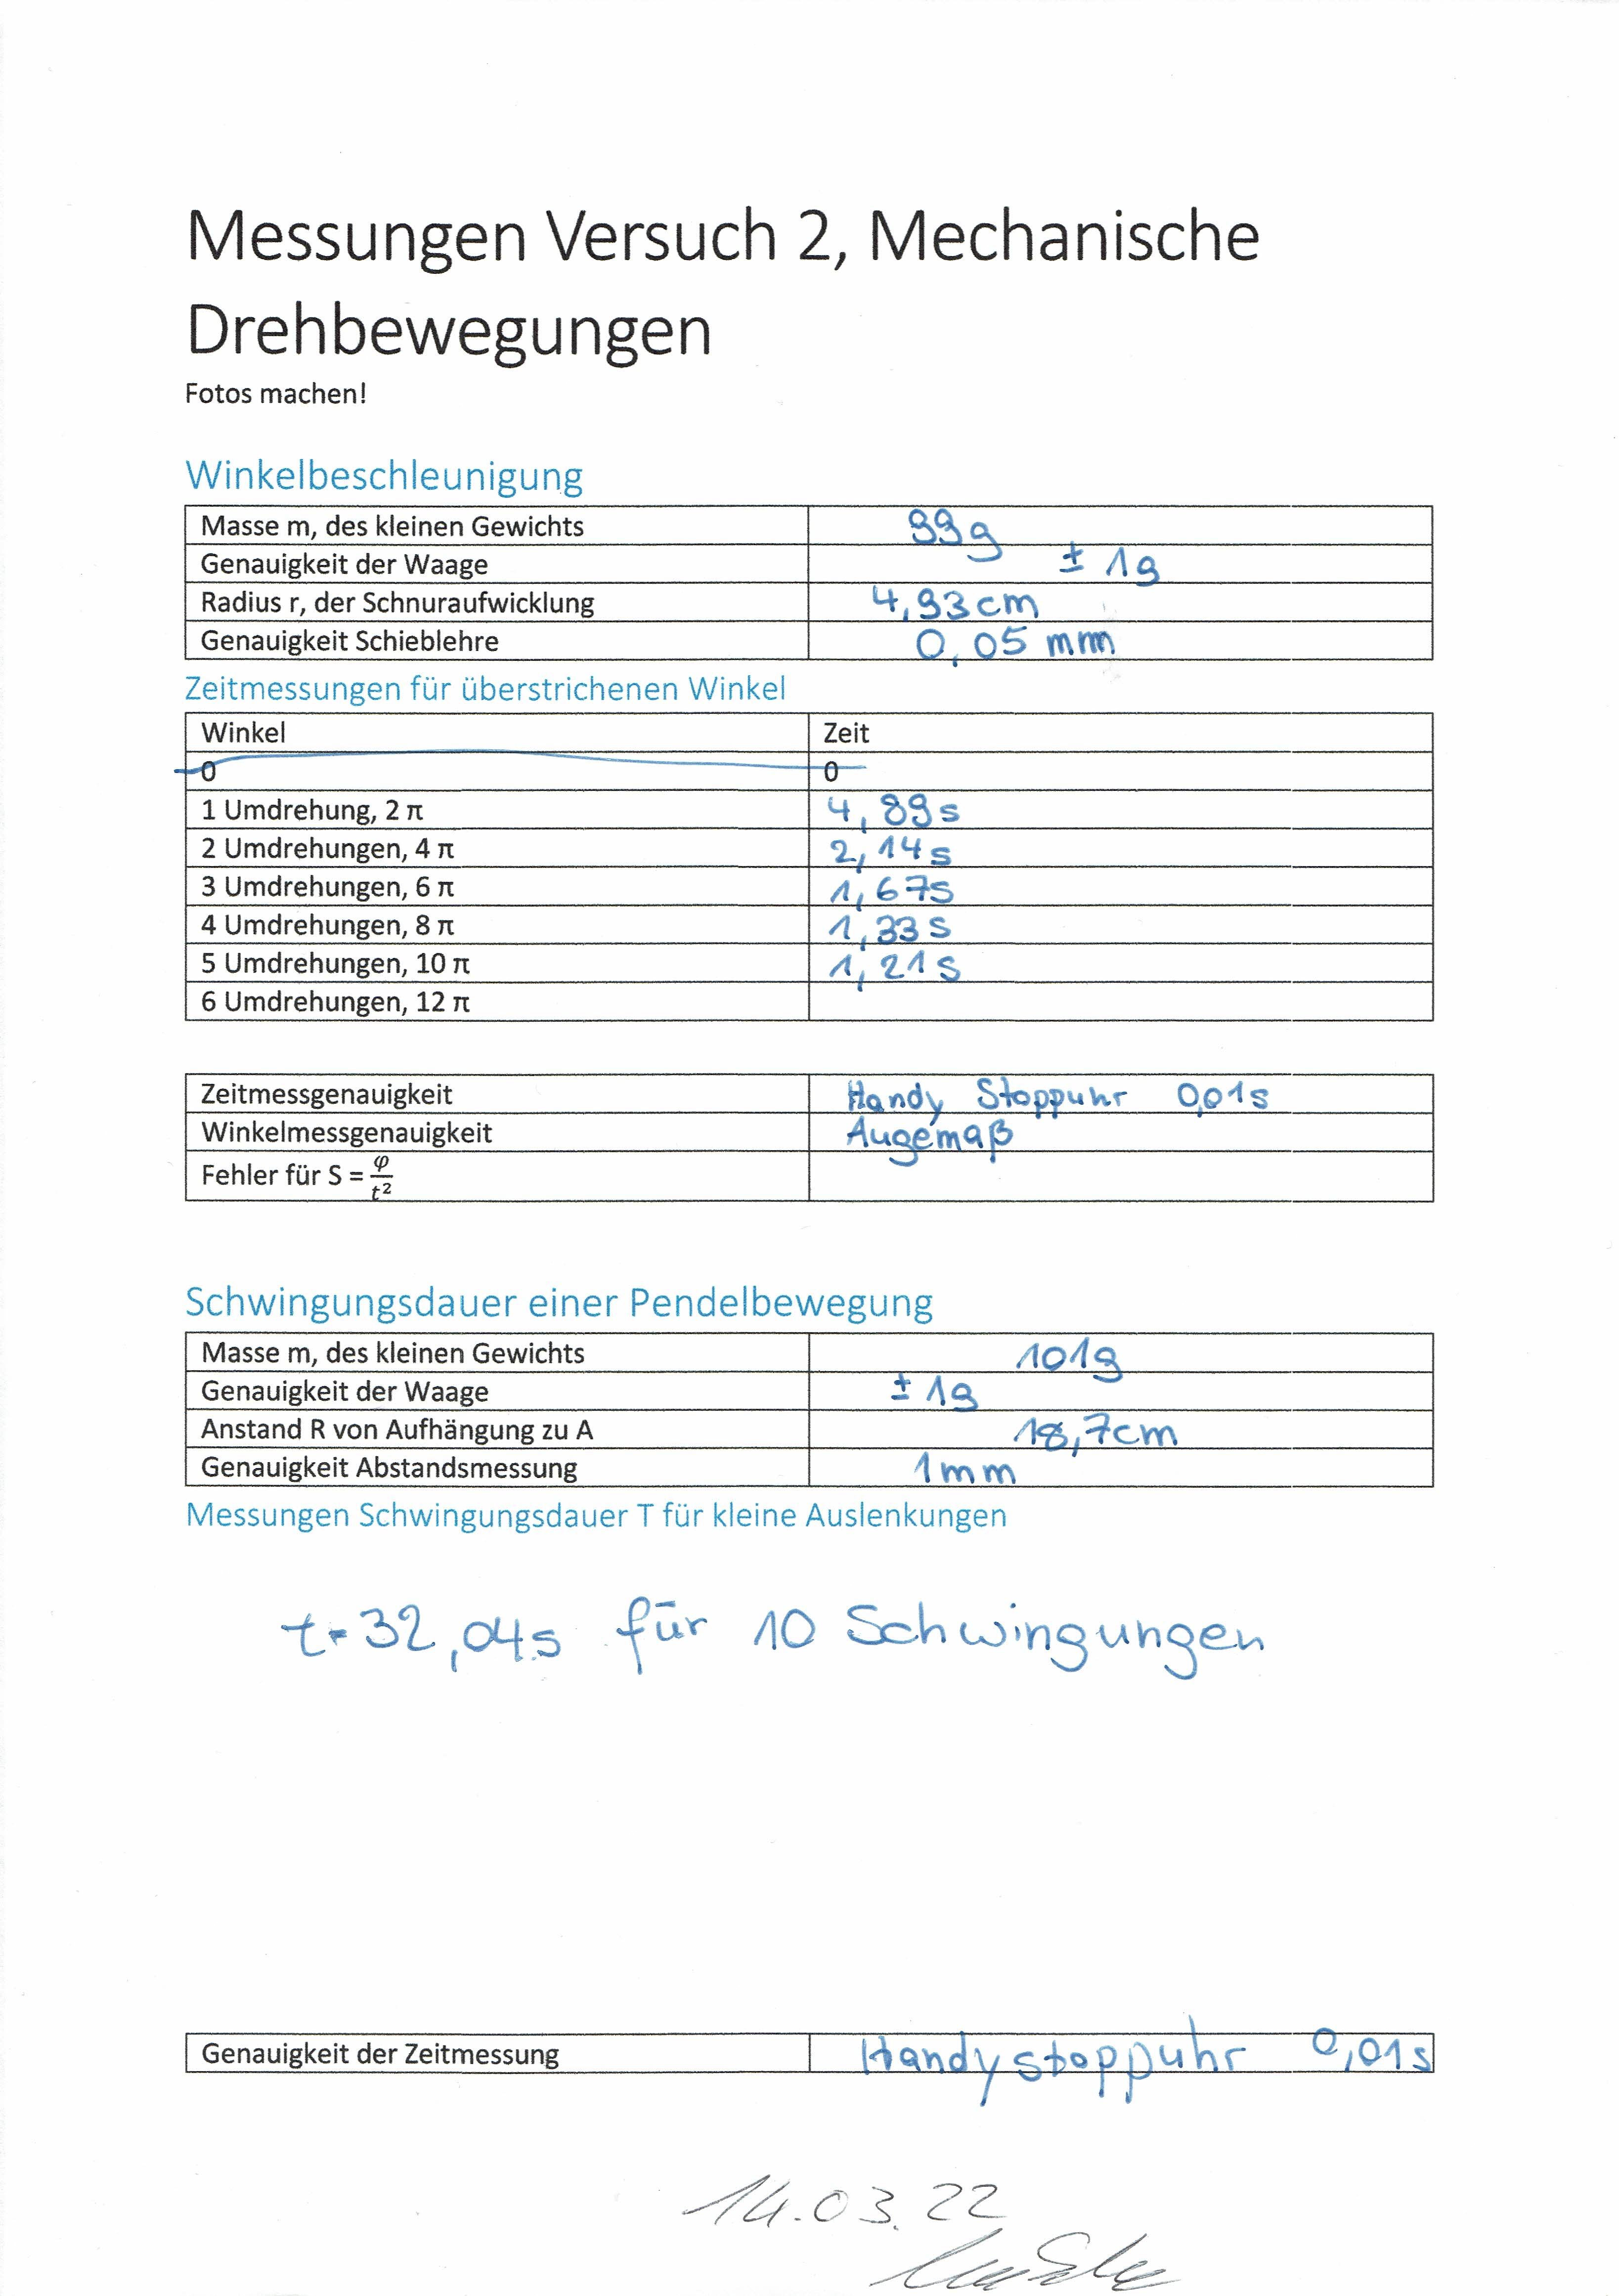
\includegraphics[height=14cm]{messwerte1.jpg}
		\caption{Messwerte der ersten beiden Teilversuche}
	\end{figure}

	\begin{figure}[!ht]\label{fig:Messwerte2}
		\centering
		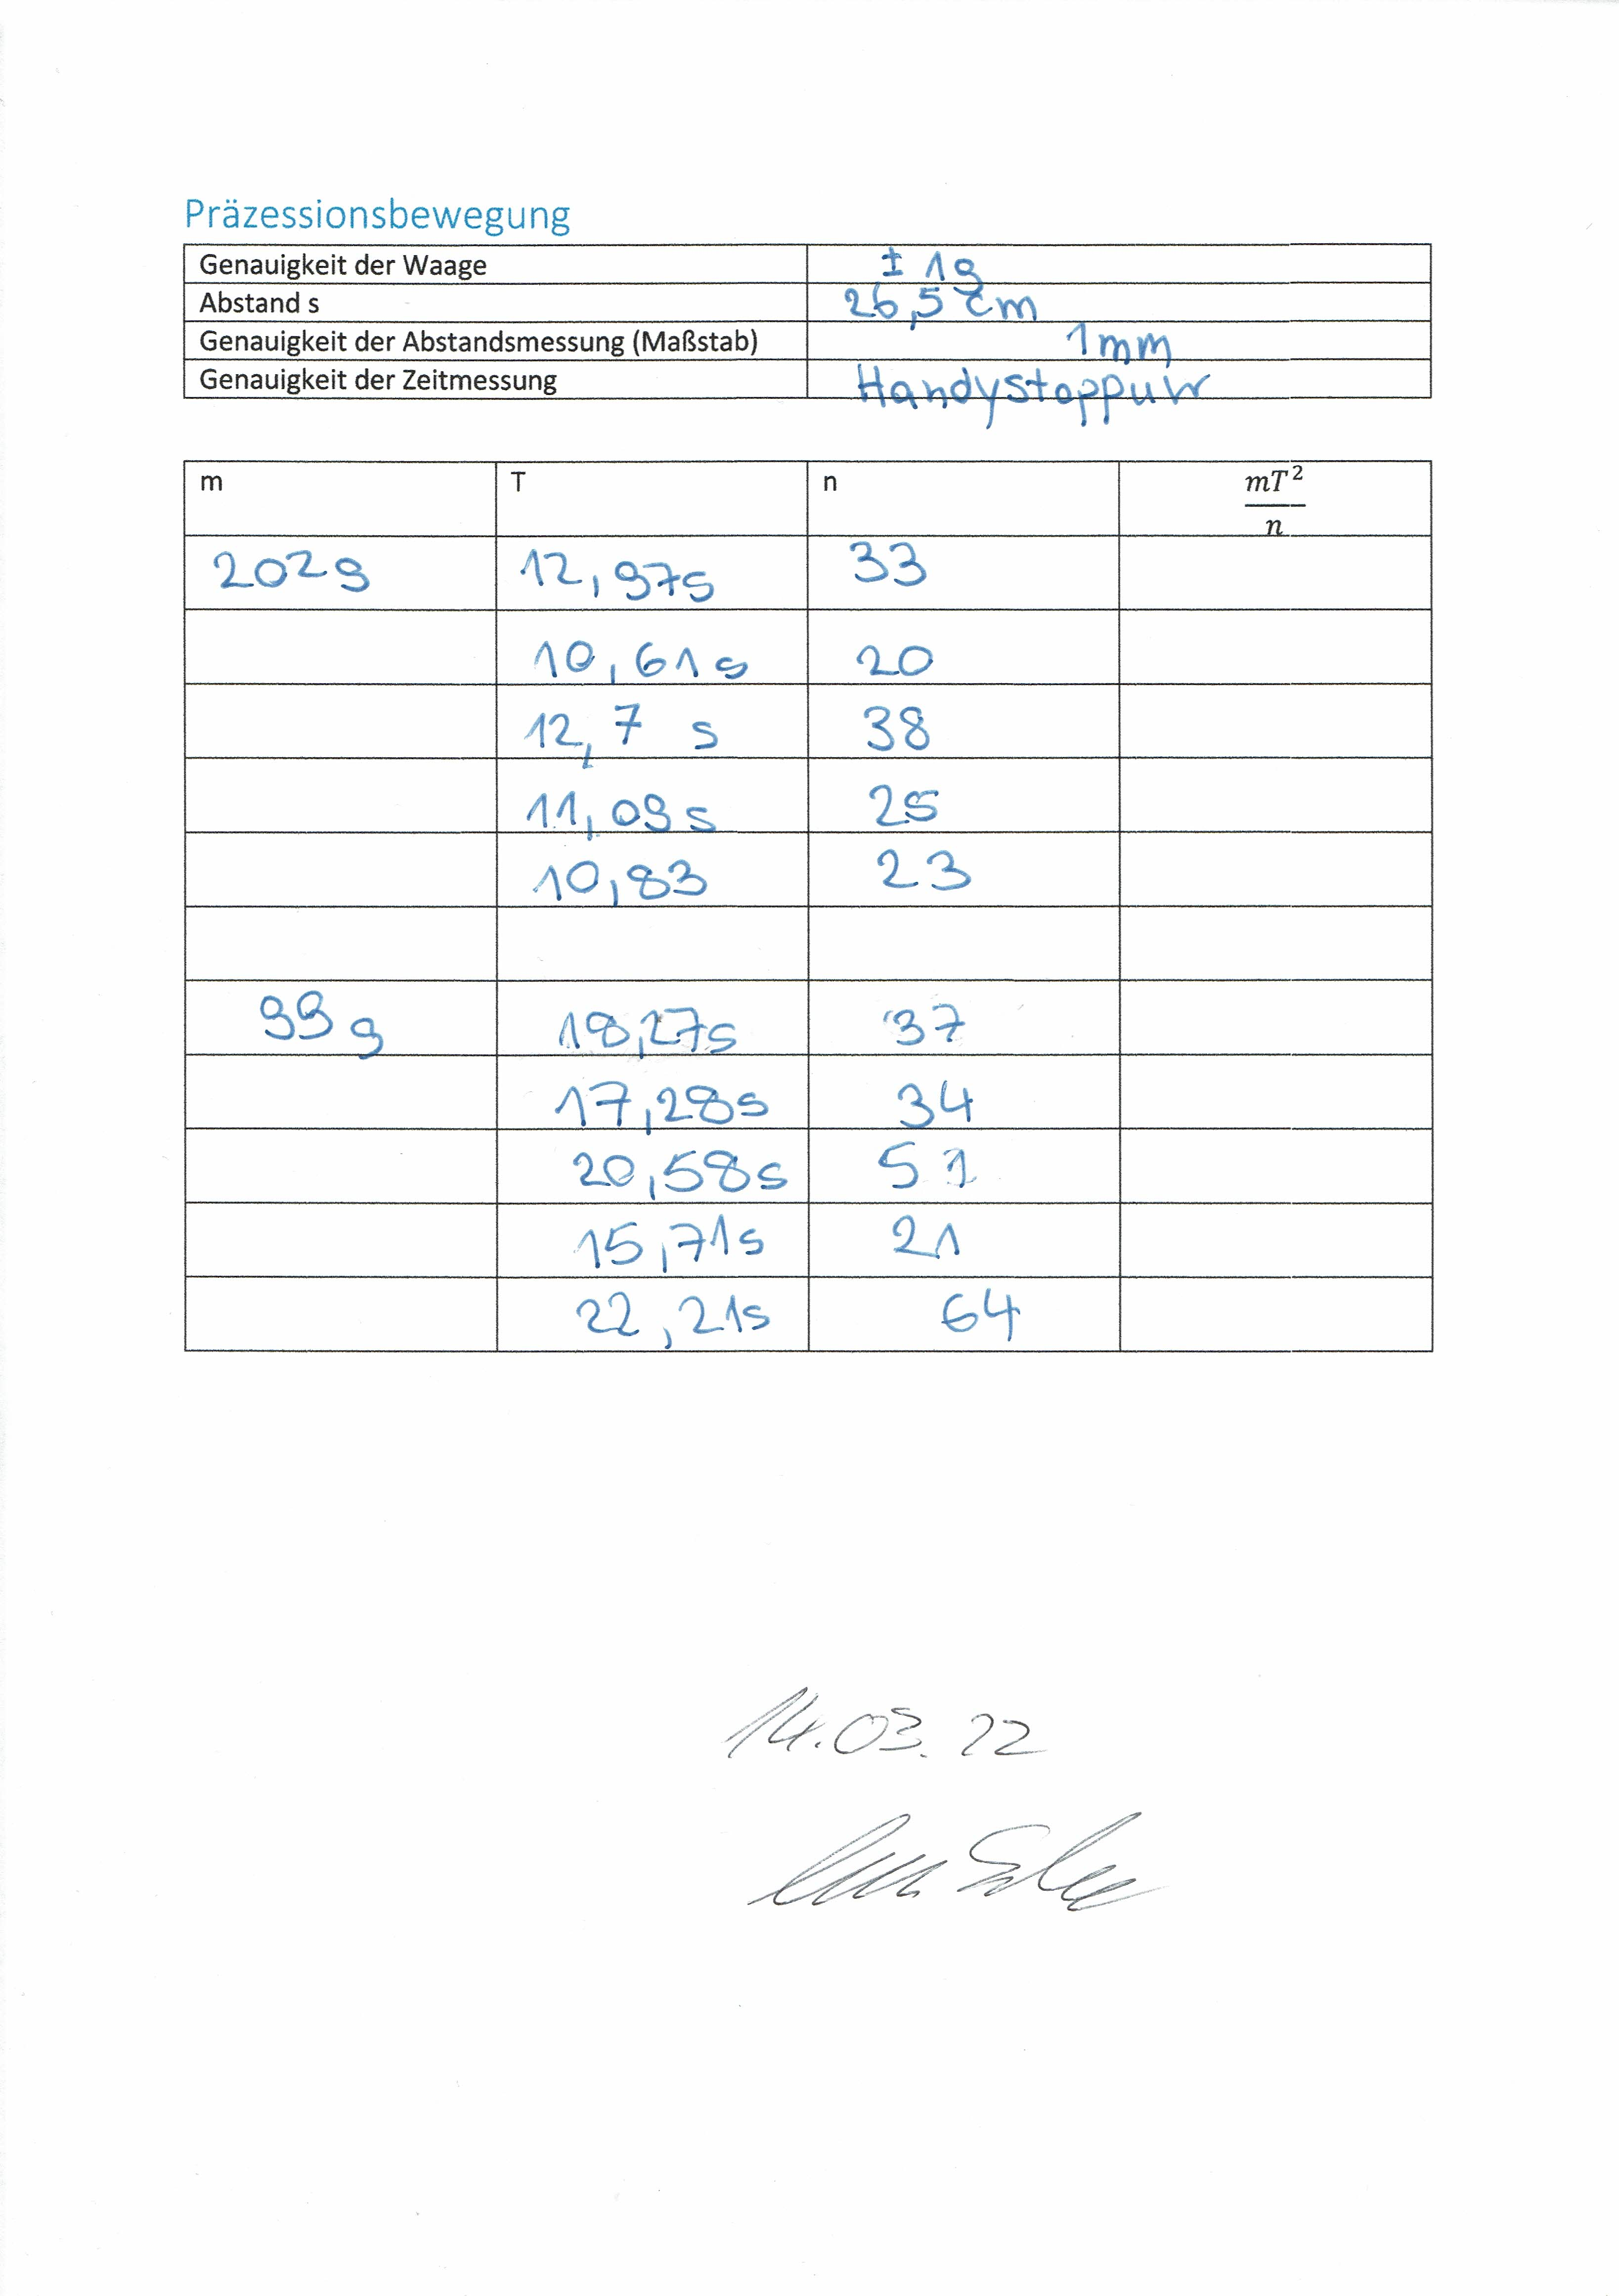
\includegraphics[height=14cm]{messwerte2.jpg}
		\caption{Messwerte des letzten Teilversuchs}
	\end{figure}

\end{document}
